\section{INTRODUCTION}
\label{sec:intro}

\renewcommand{\thefigure}{\thesection.\arabic{figure}} %setzt Nummerierung der Figure wieder auf 0 für Section
\setcounter{figure}{0}

\renewcommand{\thetable}{\thesection.\arabic{table}} %setzt Nummerierung der Table wieder auf 0 für Section
\setcounter{table}{0}


%%%%%%%%%%%%%%%%%%%%%%%%%%%%%%%%%%%%%%%
%% Add your introduction here

The pressing situation of the planets "health" is a scientific consensus \citep{ipccClimateChange20222022, planetaryboundariessciencepbsciencePlanetaryHealthCheck2025}. Already we can see the impact in our day to day live that the taken projecteries in the last years and decades are to be proven true, so we can measure for example a temperature rise in Europe of 2.5\,°C towards preindustrial times as well as a higher frequency of \gls{compound} \citep{ionitaDroughtsHotterDroughts2026, c3s/ecmwfC3SWMOEuropeanState2026}. 

So it is highly necessary to develop strategies for adaption to this changing environment, but more so for mitigation to stabilize the climate and to keep at least the 2\,°C global-goal of \textcite{unfcccParisAgreement2015}. 

One of the main driver for this development is the anthropogenic climate change. Climate change is one of nine \gls{planetaryBoundarysGLS} (\acrshort{pb}) processes that are relevant for containing a stable system on earth, to grant condition, in which human mankind can knowingly thrive \textcite{planetaryboundariessciencepbsciencePlanetaryHealthCheck2025}. Like six other of them climate change exceeded its \acrshort{pb} already (ibid.).\\

\begin{wrapfigure}{r}{0.4\textwidth}
	\centering
	
\includegraphics[width = 0.39\textwidth]{figures/Intoduction/FIGURE_21_Different_gases_and_sectors_contribute_unevenly_to_climate_change-1.jpeg}
	\caption[The share of the three main \acrshort{ghg} (\ch{CO2}, \ch{CH4}, \ch{N2O}) on the anthropogenic temperature rise since 1850.]{The share of the three main \acrshort{ghg} (\ch{CO2}, \ch{CH4}, \ch{N2O}) on the anthropogenic temperature rise since 1850. Each \acrshort{ghg} is subdivided in two groups depending on the emission source ("Agriculture and Land" or "Fossil and Industry").  Source: \citep{planetaryboundariessciencepbsciencePlanetaryHealthCheck2025}, licensed under CC BY 4.0}
	\label{fig:GHG_respons_temp_change}
\end{wrapfigure}

The relevant value for climate change is the anthropogenic \gls{radForce}, which not only exceeded the \acrshort{pb} (+1~W/m\textsuperscript{2}) 2025 but the boundary for the \gls{zoneOfIncreasingRisk} (+1.5~W/m\textsuperscript{2}) as well with a value of 2.97~W/m\textsuperscript{2} \parencite[p.\,13]{planetaryboundariessciencepbsciencePlanetaryHealthCheck2025, irfanChapterEightRadiative2024}. One strong anthropogenic influence of this value is the emission of \acrfull{ghg} \parencite{teamAnnualGreenhouseGas2025}. Very prominent is \ch{CO2} as being the most abundant (423~ppm in the atmosphere 2025) and biggest responsibility for the temperature rise of over 1.5\,°C (more than 50\%, see \cref{fig:GHG_respons_temp_change}) and change in radiative forcing \parencite{planetaryboundariessciencepbsciencePlanetaryHealthCheck2025}.\\

The second most abundant \acrshort{ghg} and with the biggest relative increase in atmospheric concentration (around 265\% from 720~ppb 1750 to 1935~ppb in 2026) is methane \parencite{appelhansUnterschatztesTreibhausgasMethan2025, planetaryboundariessciencepbsciencePlanetaryHealthCheck2025, thoningTrendsGloballyaveragedCH42022}. Methane is also responsible (see \cref{fig:GHG_respons_temp_change}) for around 30\% (\gls{gross}) of the anthropogenic temperature rise \citep[p.\,9]{appelhansUnterschatztesTreibhausgasMethan2025}. 

If compared to \ch{CO2} some features makes it highly intresting as a potential target for mitigation. 

The stronger impact of methane on radiative forcing and its relatively short lifetime in the atmosphere of 12.4~years (15-40\% of \ch{CO2} is still in the atmosphere after 1000 years) \parencite{appelhansUnterschatztesTreibhausgasMethan2025} lead to \acrlong{gwp} (\gls{gwpGls}) values that strongly decline over longer time horizonts (\gls{gwpGls}20: 79.7 and \gls{gwpGls}100: 27 for non-fossil \ch{CH4} \parencite[Table~7.15]{IPPCC_AR6_Chapter7_GWP}).

This means, as a mitigation that addresses \ch{CH4} it is enough to reduce the methane emission and within two decades a notable impact will be achieved, while for carbon dioxide strategies must also be focus the removal of \ch{CO2} from the atmosphere.\\

Right now methane is still accumulating in the atmosphere \parencite{saunoisGlobalMethaneBudget2025, thoningTrendsGloballyaveragedCH42022}. Whereas the three biggest sources globally for anthropogenic \ch{CH4} are the agriculture- (approx 40\%), energy- (36\%) and waste-sector (22\%) \parencite{appelhansUnterschatztesTreibhausgasMethan2025, mundraEmergentMethaneMitigation2024}. The emission derived from the energy and waste sector can be reduced with today's technical knowledge and options quit easily \parencite{appelhansUnterschatztesTreibhausgasMethan2025, intergovernmentalpanelonclimatechangeipccAgricultureForestryOther2022}. Emissions from agriculture, on the other hand, are counted to "hard-to-abate", because we are lacking methane reducing technologies and strategies that socially and economically accepted \parencite{appelhansUnterschatztesTreibhausgasMethan2025, edelenboschReducingSectoralHardtoabate2024, thoningTrendsGloballyaveragedCH42022, intergovernmentalpanelonclimatechangeipccAgricultureForestryOther2022}.

This is due to the fact that methane is not produced specifically through any particular economic activity but arises naturally from biological processes, primarily through enteric fermentation, especially in cattle (77\%), and manure management, together they make up for 31\% of global methane emission \parencite{appelhansUnterschatztesTreibhausgasMethan2025, smithAgriculturalMethaneEmissions2021}.\\

The only option for reducing methane emissions for this right now is to reduce the number of live stock dramatically, which is contrary to the rise of demand for livestock products and globally rising numbers of livestock \parencite{faoLivestockBalance2009, edelenboschReducingSectoralHardtoabate2024, appelhansUnterschatztesTreibhausgasMethan2025}. This bachelor thesis wants to attack this lack of options by further investigating a mitigation strategy for the largest single source of methane emissions in the agricultural sector: "immunization of cattle" against the methanogenic microbiome. For this purpose, an interdisciplinary approach was chosen with a biochemical and geographical part. \\

This interdisciplinary approach allows bringing two scales of investigation together in one work. 

The biochemistry site, on one hand, which develops new approaches to attack methane production on cellular or organism level. On the other hand, the geographical perspective, which places the results in the context of multifactorial climate change and can assess the extent to which the biochemical approach can play a role to mitigate.\\

In the following each site will have its own brief introduction.

\subsection{Biochemestry}
\label{sec:intro_biochem}

To attack methane emission from cattle it is necessary to understand where it occurs in the digestive system. Cattle as a ruminant has a rumen, or large "fore-stomach", which enables them to break down and digest long fibers of carbohydrates such as plant cells via microbial fermentation \parencite{mossMethaneProductionRuminants2000a, epaInventoryUSGreenhouse2024}. These fermentation processes carried out by a wide variety of microbes produce \ch{H2} and \ch{CO2}, which must be removed as quickly as possible due to negative feedback inhibition of fermentation. Put simply, this can be achieved by acetogenic microbes, which produce short-chain hydrocarbons, or by methanogenic archaea, which produce \ch{CH4} \parencite{boadiMitigationStrategiesReduce2004, garnettGreenhousegasAbatementAustralian2024}. \\

In the rumen, methanogenic archaea are often the dominant group, as they can metabolize \ch{H2} and \ch{CO2} more efficiently \parencite{mossMethaneProductionRuminants2000a}. This also means that completely eliminating methanogenic \gls{archa} would not be advisable—if even possible—since, according to \textcite{morvanEstablishmentHydrogenutilizingBacteria1994}, \ch{H2} would accumulate, making digestion in cattle less efficient.

However, the goal of the immunization strategy is to shift the microbiome toward a higher proportion of acetogenic bacteria by training the cattle’s immune system to recognize and attack methanogenic archaea \parencite{malyuginaMitigationStrategiesMethane2025}. This would result, on the one hand, in less methane production and, on the other hand, in the production of more short-chain hydrocarbons that can still be digested and absorbed by the cattle. In theory, this would also lead to more efficient digestion \parencite{boadiMitigationStrategiesReduce2004, mossMethaneProductionRuminants2000a, malyuginaMitigationStrategiesMethane2025}.\\

Already, there were some experiments trying to immunize cattle against methanogenic \gls{archa} with a inactivated vaccine with low and inconsistent success, mainly due high surface variability of methanogens  \parencite{wrightReducingMethaneEmissions2004, malyuginaMitigationStrategiesMethane2025}.

To solve this problem a robust and specific antigen has to be found for the dominant methanogen species. The problem here, however, is that while the composition of methanogenic archaea in the rumen is now somewhat better understood (four main groups and the dominant genus is \acrfull{mbrevi}, which accounts for approximately 60\% of methanogenic archaea \parencite[p.\,3]{baca-gonzalezAreVaccinesSolution2020}), the individual species remain poorly understood and characterized, even though some of them have already been isolated \citep{baca-gonzalezAreVaccinesSolution2020}.\\

Here, the strains \acrfull{thau} and \acrfull{bovi} isolated from the rumen of cattle will be further investigated \parencite{millerDescriptionMethanobrevibacterGottschalkii2002, leeMethanobrevibacterBoviskoreaniSp2013}. For this purpose, the investigation will have two sites.\\

First, general analyses and cultivation characterization as cell-count per ml or checking if they grow on solid media.

Second, trying to implement for the first time a genetic tool for \acrlong{mbrevi}. Following the approach of \textcite{kleinMarkerlessMutagenesisEnables2025} for \textit{Methanothermobacter marburgensis}, plan is to transform \acrlong{mbrevi} via interdomain conjugation with \acrfull{ecol}. Therby a \gls{suicide} was used, with four main parts (see \cref{fig:general_plasmid_map}):
\begin{itemize}
	\item \acrshort{ecol} casette with an \gls{ori} and a selection via chloramphenicol resistance plus the \textit{traJ} as relevant gen for the conjugation
	\item Promoter region containing the \textit{pac} gene, which serves as a selection marker for the transformed \acrshort{mbrevi} with \acrfull{puro}
	\item Homology arms, where the segments of the \acrfull{gDna} from the transforming \acrshort{mbrevi} are located. The homology regions flank the gene to be deleted. Through single homologous recombination events, the plasmid is first integrated and then removed again via counterselection, whereby the gene flanked by the homology arms is also excised \parencite{kleinMarkerlessMutagenesisEnables2025}.
	\item The \acrfull{hpt} gene ensures sensitivity to \acrfull{azaeight}
\end{itemize}


\begin{figure}[!h]
	\centering
	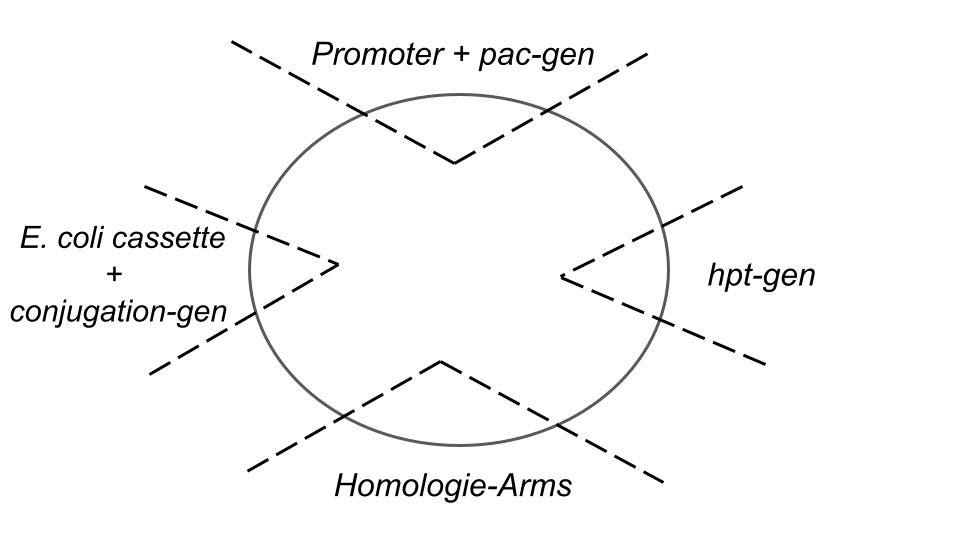
\includegraphics[width = 0.75\textwidth]{figures/Results/BC/Allgemeiner_grober_aufbau_plasmide}
	\caption[Sketch of the general structure of the suicide plasmids for the transformation of \acrfull{thau} and \acrfull{bovi} via conjugation using \textcolor{red}{\acrshort{ecol}}.]{Sketch of the general structure of the suicide plasmids for the transformation of \acrfull{thau} and \acrfull{bovi} via conjugation using \textcolor{red}{\acrshort{ecol}}.
	The plasmid contains the \acrshort{ecol} cassette with \gls{ori} and \textit{catp} as a selection marker using chloramphenicol, as well as the conjugation gene \textit{traJ}.
	In addition, all plasmids contain the \textit{hpt} gene to enhance counterselection and the two homology arms that flank the genomic \textit{hpt} gene of the corresponding organism. The final important region is the one containing the \textit{pac} gene and its associated promoter, which serves as a selection marker.},
	\label{fig:general_plasmid_map}
\end{figure}

In the following experiments, regions on the homology arms are selected that flank the \textit{\acrshort{hpt}} of the respective organism, resulting in a mutant lacking genomic \textit{\acrshort{hpt}}. This makes it possible to target any other gene in the genome by selecting the appropriate homology regions and removing them via markerless counterselection \parencite{kleinMarkerlessMutagenesisEnables2025}.

\subsection{Geography}

DE has a-non linear relation towards GE (see \cref{eq:GE_berechnung}:\ref{eq:REG_calculation}). 



Muss Tier 1 und 2 von IPCC erläutern, so wie insgesamt IPCC
